\chapter{Reactor semicontinuo mezcla perfecta}
\section{Introducción}
\begin{flushleft}
    En estos reactores, los caudales de entrada y salida difieren, lo que genera variaciones en el volumen de operación. Las configuraciones más habituales consisten en la ausencia de una de estas corrientes: si no hay entrada, el reactor se vacía progresivamente; si no hay salida (el caso más común), el volumen aumenta a medida que se adicionan reactivos sobre una carga inicial.\\
    \vspace{1em}
    El reactor semicontinuo de mezcla perfecta es de especial interés en reacciones múltiples donde se busca maximizar la selectividad hacia el producto deseado. Asimismo, es fundamental en procesos altamente exotérmicos, ya que permite dosificar un reactivo a velocidad controlada para garantizar la estabilidad energética del sistema.\\
    \vspace{1em}
    Para su análisis, se definirá la importancia de la configuración del reactor y su modo de funcionamiento:
\end{flushleft}

\dfn{Magnitudes a trabajar}{\begin{itemize}
        \item Selectividad
              \begin{enumerate}
                  \item local definida en estado estacionario
                  \item instantanea en estado no estacionario
              \end{enumerate}
              \begin{equation}
                  \text{Selectividad} = s = \frac{\text{Velocidad de transformación de A en P}}{\text{Velocidad total de transformación de A}}
              \end{equation}
              se define para una reaccion A + $\dots \to \alpha_p$ P + $\dots$  de forma que queda tal que:
              \begin{equation}
                  s = \frac{r_p/\alpha_p}{r_A}
              \end{equation}
        \item Selectividad global tambien conocida como $S_G$ debido a que es mas facil trabajar con moles que con la velocidad de reacción:
              \begin{equation}
                  S_G = \frac{\text{moles de A transformado en P}}{\text{moles de A transformados}}
              \end{equation}
        \item Conversión global $X_G$
              \begin{equation}
                  X_G=\frac{\text{moles de A transformados}}{\text{moles de A alimentados}}
              \end{equation}
        \item Rendimiento global $R_G$:
              \begin{equation}
                  R_G = \frac{\text{moles de A transformados en P}}{\text{moles de A alimentados}}
              \end{equation}
        \item es evidente que la relacion entre las 3 magnitudes es: $R_G = S_G \cdot X_G$
    \end{itemize}}

\section{Relacion entre selectividades en reactores}
\subsection{Reactor discontinuo mezcla perfecta}
\noindent En una reacción $A + \dots \to \alpha_p P + \dots$  recordando que para el reactor discontinuo mezcla perfecta teniamos los balances:
\begin{equation}
    \left.
    \begin{aligned}
        \frac{dN_A}{dt} & = -r_A \cdot V \\[10pt]
        \frac{dN_P}{dt} & = r_P \cdot V
    \end{aligned}
    \right\} \implies \frac{dN_P}{dN_A} = -\frac{r_P}{r_A}
    \label{eq:Sg_rdmp}
\end{equation}
lo que se ha hecho es calcular la variacion de los moles de P respecto a los moles de A \textbf{(selectividad)}, es decir dividir la expresión de arriba con la de abajo, que da la expresión de la derecha.
ahora si aplicamos el concepto de la selectividad global para este caso:

\begin{equation}
    S_G = \frac{\textcolor{blue}{\left(N_{Pf}-N_{P0}\right)/\alpha_P}}{\textcolor{red}{N_{Af}-N_{A0}}} = \textcolor{red}{\frac{1}{(N_{A0}-N_{Af})}}\textcolor{blue}{\int_{N_{A0}}^{N_{Af}}\left(\frac{dN_P/\alpha_P}{dN_A}\right)dN_A}
\end{equation}

\nt{Como se ha señalado en rojo, al tratarse de un intervalo sin variación, la relación puede expresarse de forma algebraica (tanto antes como después del signo igual). Por el contrario, la sección en azul representa una variación decreciente a lo largo del proceso; por tanto, la única forma de calcularla con precisión es mediante el uso de la integral}

ahora si reordenamos e introducimos el resultado obtenido de la ecuación ~\eqref{eq:Sg_rdmp}:

\begin{equation}
    S_G = \frac{1}{N_{A0}-N_{Af}}\int_{N_{A0}}^{N_{Af}}\left(\frac{r_P/\alpha_P}{r_A}\right)dN_A \rightarrow \boxed{S_G=\frac{1}{N_{A0}-N_{Af}}\int_{N_{A0}}^{N_{Af}}s \, dN_A}
\end{equation}

\noindent Además en el caso de $\rho$ = $\text{cte}$ se mantiene el volumen constante y por tanto se puede expresar en función de las concentraciones:

\begin{equation}
    \boxed{S_G = \frac{1}{C_{A0}-C_{Af}}\int_{C_{A0}}^{C_{Af}}s \, dC_A}
\end{equation}

\subsection{Reactor continuo flujo de pistón}
de forma analoga el balance generico para el flujo de pistón era:

\begin{equation}
    \frac{dN_i}{dt} = ni - (ni+dni) + r_i dV \cdot dV
\end{equation}
\noindent para el estado estacionario se queda en: \\
\begin{equation}
    \left.
    \begin{aligned}
        -\frac{dn_A}{dV} & = r_A \\[10pt]
        \frac{dn_P}{dV}  & = r_P
    \end{aligned}
    \right\} \implies \frac{dn_P}{dn_A} = -\frac{r_P}{r_A}
    \label{eq:Sg_pfr}
\end{equation}

\noindent la variación del caudal molar de p respecto el caudal molar vendria en funcion de las velocidades, la expresión es analoga a los reactores discontinuos como se vio en el apartado anterior, la selectividad global se vuelve a definir como:

\begin{equation}
    S_G = \frac{\textcolor{blue}{\left(n_{Pf}-n_{P0}\right)/\alpha_P}}{\textcolor{red}{n_{Af}-n_{A0}}} = \textcolor{red}{\frac{1}{(n_{A0}-n_{Af})}}\textcolor{blue}{\int_{n_{A0}}^{n_{Af}}\left(\frac{dn_P/\alpha_P}{dn_A}\right)dN_A}
\end{equation}
\newpage

\noindent y luego igual que en el reactor discontinuo se llega a las mismas expresiones pero en caudales molares:

\begin{equation}
    S_G = \frac{1}{n_{A0}-n_{Af}}\int_{n_{A0}}^{n_{Af}}\left(\frac{r_P/\alpha_P}{r_A}\right)dn_A \rightarrow \boxed{S_G=\frac{1}{n_{A0}-n_{Af}}\int_{n_{A0}}^{n_{Af}}s \, dn_A}
\end{equation}

\noindent y con $\rho$ = $\text{cte}$ se mantiene el volumen constante y por tanto se puede expresar en función de las concentraciones:

\begin{equation}
    \boxed{S_G = \frac{1}{C_{A0}-C_{Af}}\int_{C_{A0}}^{C_{Af}}s \, dC_A}
\end{equation}

\subsection{Reactor continuo mezcla perfecta}
\noindent Buscando la relación entre selectividd global y global de forma analoga a los casos anteriores:

\begin{equation}
    \frac{dN_i}{dt} = n_{i0} - n_{if} + r_i\cdot V
\end{equation}
\noindent Aplicando este balance a los componentes A y P en estado estacionario:
\begin{equation}
    \left\{
    \begin{aligned}
        n_{A0} - n_{Af} & = (r_{A})_f \, V     \\[6pt]
        n_{Pf} - n_{P0} & = -\, (r_{P})_f \, V
    \end{aligned}
    \right.
    \label{eq:Sg_rcmp}
\end{equation}
\noindent Si tenemos en cuenta la definición de la selectividad global queda de la siguiente forma:
\begin{equation}
    S_G = \frac{(n_{Pf}-n_{P0})/\alpha_P}{n_{A0}-n_{Af}} = \frac{-(r_P)_f/\alpha_P}{(r_A)_f} = S_f
\end{equation}
\nt{En este tipo de reactor la selectividad global es la selectividad final de salida del reactor.}

\section{Influencia del orden de reacción}

En un sistema de reacciones múltiples:

\begin{itemize}
    \item $ A \rightarrow P$  \hspace{2mm} $r_1$ = $r_p$ = $k_1 \cdot C_A^{n_1}$
    \item $A \rightarrow Q$ \hspace{2mm} $r_2$ = $r_q$ = $k_2 \cdot C_A^{n_2}$
\end{itemize}

\nt{A es el reactivo limitante P el producto deseado y Q el producto no deseado}
\begin{flushleft}
    la selectividad del proceso, es decir la velocidad de reacción de A para dar P dividido por la velocidad de transformación de A seria la siguiente:
    \begin{equation}
        s = \frac{r_1}{r_1 + r_2}
        = \frac{1}{1 + \frac{r_2}{r_1}}
        \quad \text{sustituyendo } r_i \quad
        = \frac{1}{1 + \frac{k_2}{k_1} \, C_A^{n_2 - n_1}}
    \end{equation}
\end{flushleft}
\noindent como obviamente queremos maximizar la selectividad para tener la mayor cantidad de P, nos tenemos que fijar en el denominador, donde queremos que $C_A^{n_2-n_1}$ sea lo mas pequeño posible, para ello se tiene en cuenta lo siguiente:
\begin{itemize}
    \item Si $n_2 > n_1$ imaginemos que $n_1 = 1$ y $n_2 = 2$, entonces $n_2 - n_1 = 1$ y tendriamos: $\frac{1}{1 + \frac{k_2}{k_1} \, C_A}$
    \item Si $n_2 < n_1$ imaginemos que $n_1 = 2$ y $n_2 = 1$, entonces $n_2 - n_1 = -1$ y tendriamos: $\frac{1}{1 + \frac{k_2}{k_1} \, \frac{1}{C_A}}$
\end{itemize}
\subsection{Primer caso n1 < n2}
\noindent Para ver como afecta lo analizamos segun el tipo de reactor:
\subsubsection{Flujo pistón}
\begin{equation}
    S_G= \frac{1}{C_{A0}-C_{Af}}
    \int_{C_{A0}}^{C_{Af}} \frac{1}{1 + \frac{k_2}{k_1} \, C_A}\, dC_A
\end{equation}
\begin{equation}
    \text{Sea } u = 1 + \frac{k_2}{k_1} C_A
    \quad \Rightarrow \quad
    \frac{du}{dC_A} = \frac{k_2}{k_1}
    \quad \Rightarrow \quad
    dC_A = \frac{k_1}{k_2} \, du
\end{equation}
\noindent La selectividad global ($S_G$) se obtiene integrando la selectividad instantánea respecto a la concentración en el intervalo de operación:

\begin{equation}
    S_G = \frac{1}{C_{A0}-C_{Af}} \int_{C_{A0}}^{C_{Af}} \frac{1}{1 + \frac{k_2}{k_1} C_A} dC_A
\end{equation}

\noindent Al resolver la integral, es necesario compensar la \textbf{derivada interna} del argumento ($a = \frac{k_2}{k_1}$), lo que hace aparecer el factor recíproco \textcolor{red}{$\frac{k_1}{k_2}$} fuera del logaritmo:

\begin{equation}
    S_G = \frac{1}{C_{A0}-C_{Af}} \cdot \textcolor{red}{\frac{k_1}{k_2}} \left[ \ln \left( 1 + \frac{k_2}{k_1} C_A \right) \right]_{C_{A0}}^{C_{Af}}
\end{equation}

\noindent Evaluando los límites de integración e introduciendo la definición de conversión:

\begin{equation}
    S_G = \frac{1}{C_{A0}-C_{A0}\cdot (1-X_f)} \cdot \frac{k_1}{k_2} \ln \left( \frac{1 + \frac{k_2}{k_1}C_{A0}}{1 + \frac{k_2}{k_1}C_{A0}\cdot (1-X_f)} \right)
\end{equation}
\noindent simplificando la expresion obtenemos:
\begin{equation}
    S_G = \frac{k_1}{k_2 C_{A0}X_f} \ln \left( \frac{1 + \frac{k_2}{k_1}C_{A0}}{1 + \frac{k_2}{k_1}C_{A0}\cdot (1-X_f)} \right)
\end{equation}

\subsubsection{Reactor continuo mezcla perfecta}
\begin{equation}
    S_G= s_f = \frac{1}{1 + \frac{k_2}{k_1}C_{Af}}
    = \frac{1}{1 + \frac{k_2}{k_1}C_{A0}(1-X_f)}
\end{equation}
\begin{figure}[h]
    \begin{center}
        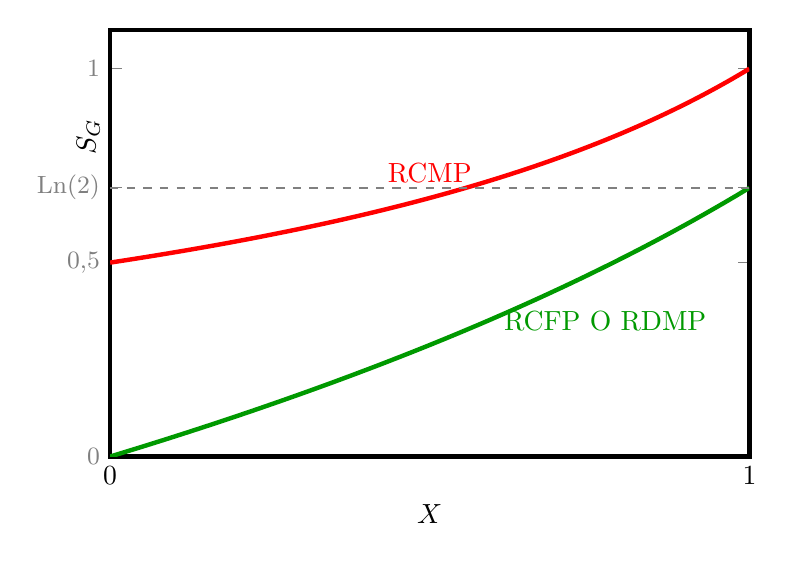
\begin{tikzpicture}
            \begin{axis}[
                    width=0.8\textwidth, height=7cm,
                    xmin=0, xmax=1, ymin=0, ymax=1.1,
                    xlabel={$X$}, ylabel={$S_G$},
                    ylabel style={
                            at={(axis description cs:0, 0.75)},
                            anchor=south,
                            rotate=0
                        },
                    yticklabel style={font=\small, color=gray},
                    axis line style={ultra thick},
                    ytick={0, 0.5, 0.693, 1},
                    yticklabels={0, {0,5}, {Ln(2)}, 1},
                    xtick={0, 1},
                    thick
                ]
                % Curva Roja (RCMP): s_f = 1 / (2-X)
                \addplot[red, ultra thick, domain=0:1, samples=100] {1 / (2 - x)};
                \node[red, anchor=south] at (axis cs: 0.5, 0.68) {RCMP};

                % Curva Verde (RCFP): ln( 2 / (2-X) ) -> Esto es lo que dibujó ella
                \addplot[green!60!black, ultra thick, domain=0:1, samples=100] {ln( 2 / (2 - x) )};
                \node[green!60!black, anchor=north west] at (axis cs: 0.6, 0.4) {RCFP O RDMP};

                % Línea guía Ln(2)
                \draw[gray, dashed] (axis cs: 0, 0.693) -- (axis cs: 1, 0.693);
            \end{axis}
        \end{tikzpicture}
        \caption{Selectividad global vs Conversion para el caso $n_1 < n_2$}
        \label{fig:RSMP_nx_n1<n2}
    \end{center}
\end{figure}

\nt{\textbf{Conclusión:} El RCMP es mas selectivo cuando la reaccion que da el producto deseado tiene un menor orden cinético.}

\subsection{Segundo caso $n_1 > n_2$}
\noindent Para este escenario, la selectividad instantánea se ve favorecida por concentraciones elevadas de reactivo. Analizamos el comportamiento según el diseño del reactor:

\subsubsection{Flujo pistón (RCFP)}
\noindent La selectividad global ($S_G$) en un reactor de flujo pistón se define como el promedio integral de la selectividad instantánea:
\begin{equation}
    \boxed{ S_G = \frac{1}{C_{A0}-C_{Af}} \int_{C_{A0}}^{C_{Af}} s\cdot dC_A }
\end{equation}
\begin{equation}
    S_G = \frac{1}{C_{A0}-C_{Af}} \int_{C_{A0}}^{C_{Af}} \frac{1}{1 + \frac{k_2}{k_1} \underbrace{C_A^{-1}}_{1/C_A}} dC_A
\end{equation}

\noindent Para resolver esta integral de forma sencilla, aplicamos un artificio algebraico multiplicando y dividiendo por $C_A$:

\begin{equation}
    S_G = \frac{1}{C_{A0}-C_{Af}} \int_{C_{A0}}^{C_{Af}} \frac{C_A}{C_A + \frac{k_2}{k_1}} dC_A
\end{equation}
\noindent Ahora mediante un procedimiento sencillo obtenemos la expresión de la integral:
\begin{enumerate}
    \item \textbf{suma y resta}: Sumamos y restamos el término \textcolor{red}{$\frac{k_2}{k_1}$} en el numerador para poder separar la fracción:
          \begin{equation}
              S_G = \frac{1}{C_{A0}-C_{Af}} \int_{C_{Af}}^{C_{A0}} \frac{C_A \textcolor{red}{ + \frac{k_2}{k_1} - \frac{k_2}{k_1}}}{C_A + \frac{k_2}{k_1}} dC_A
          \end{equation}

    \item \textbf{Separación en dos fracciones}: Dividimos el integrando en dos partes. La primera parte se simplifica a la unidad:
          \begin{equation}
              S_G = \frac{1}{C_{A0}-C_{Af}} \int_{C_{Af}}^{C_{A0}} \left(\textcolor{darkgreen}{\frac{C_A + \frac{k_2}{k_1}}{C_A + \frac{k_2}{k_1}}} -\textcolor{blue}{\frac{\frac{k_2}{k_1}}{C_A + \frac{k_2}{k_1}}} \right) dC_A
          \end{equation}

    \item \textbf{Expresión final simplificada}: Obtenemos la ecuación lista para ser integrada:
          \begin{equation}
              S_G = \frac{1}{C_{A0}-C_{Af}} \int_{C_{Af}}^{C_{A0}} \left( \textcolor{darkgreen}{\mathbf{1}} - \textcolor{blue}{\frac{\frac{k_2}{k_1}}{C_A + \frac{k_2}{k_1}}} \right) dC_A
          \end{equation}
    \item{\textbf{Resolucion integral}}
          \begin{equation}
              S_G = \frac{1}{C_{A0}-C_{Af}} \left[ \textcolor{darkgreen}{C_A} - \textcolor{blue}{\frac{k_2}{k_1} \ln\left(C_A + \frac{k_2}{k_1}\right)} \right]_{C_{Af}}^{C_{A0}}
          \end{equation}
    \item{\textbf{Evaluamos los limites:}}
          \begin{equation}
              S_G = \textcolor{red}{\frac{1}{C_{A0}-C_{Af}}} \left[ \textcolor{red}{C_{A0}-C_{Af}} - \textcolor{darkgreen}{\frac{k_2}{k_1}} \ln\left(\frac{C_{A0} + \frac{k_2}{k_1}}{C_{Af} + \frac{k_2}{k_1}}\right) \right]
          \end{equation}
          \nt{la diferencia de logaritmos se ha expresado directamente como la división de los argumentos}
    \item \textbf{Se pone en función de conversión:}
          \begin{equation}
              S_G = \textcolor{red}{1} - \frac{\textcolor{darkgreen}{k_2}}{\textcolor{darkgreen}{k_1} \cdot \textcolor{red}{C_{A0} (1-X_f)}} \ln \left( \frac{C_{A0} + \frac{k_2}{k_1}}{C_{A0}(1-X_f) + \frac{k_2}{k_1}} \right)
          \end{equation}
    \item{Multiplicamos y dividimos por $C_{A0}$ en el logartimo y sacamos factor comun}
          \begin{equation}
              S_G = 1 - \frac{k_2}{k_1 C_{A0} X_f} \ln \left( \frac{1 + \dfrac{k_2}{k_1 C_{A0}}}{(1-X_f) + \dfrac{k_2}{k_1 C_{A0}}} \right)
          \end{equation}
\end{enumerate}


\subsubsection{Reactor continuo mezcla perfecta (RCMP)}
\noindent En este caso, la selectividad global coincide con la instantánea evaluada a la concentración de salida, que es la más baja del sistema:

\begin{equation}
    S_G = \frac{1}{1 + \frac{k_1}{k_2\cdot C_{A0} \cdot (1-X_f)} }
\end{equation}
\begin{figure}[H]
    \begin{center}
        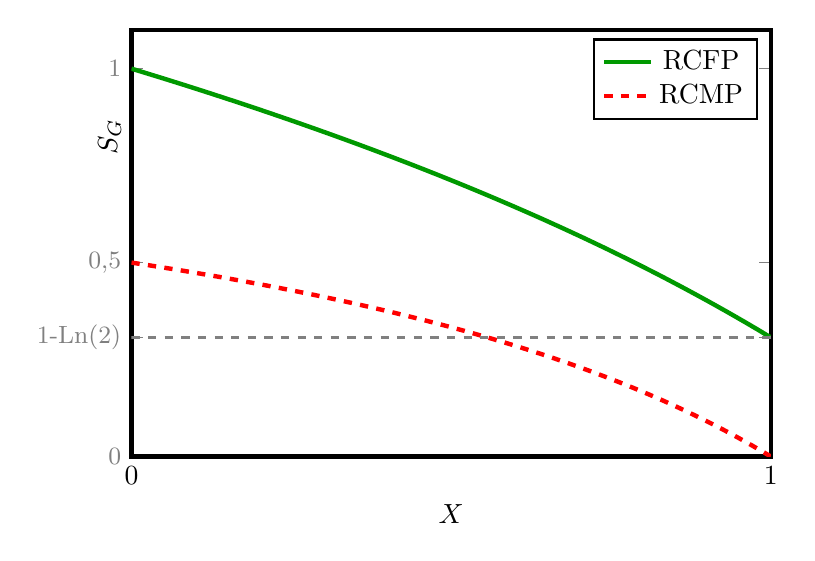
\begin{tikzpicture}
            \begin{axis}[
                    width=0.8\textwidth, height=7cm,
                    xmin=0, xmax=1, ymin=0, ymax=1.1,
                    xlabel={$X$}, ylabel={$S_G$},
                    ylabel style={
                            at={(axis description cs:0, 0.75)},
                            anchor=south,
                            rotate=0
                        },
                    yticklabel style={font=\small, color=gray},
                    axis line style={ultra thick},
                    ytick={0, 0.307, 0.5,1},
                    yticklabels={0, {1-Ln(2)}, {0,5}, 1},
                    xtick={0, 1},
                    thick,
                    legend style={anchor=north east}
                ]
                % Curva Verde (RCFP): 1 - (1/x)*ln(2/(2-x))
                % Representa la selectividad global analítica para k1=k2=Ca0=1
                \addplot[green!60!black, ultra thick, domain=0:1, samples=100] {1 - ln( 2 / (2-x) )};
                \addlegendentry{RCFP}

                % Curva Roja (RCMP): (1-x)/(2-x)
                \addplot[red, ultra thick, dashed, domain=0:1, samples=100] {(1-x)/(2-x)};
                \addlegendentry{RCMP}

                % Línea guía asintótica 1-Ln(2)
                \draw[gray, dashed] (axis cs: 0, 0.307) -- (axis cs: 1, 0.307);
            \end{axis}
        \end{tikzpicture}
    \end{center}
    \caption{Comparativa de selectividad para $n_1 > n_2$}
    \label{fig:RSMP_nx_n1>n2}
\end{figure}

\nt{\textbf{Conclusión:} Cuando $n_1 > n_2$, el \textbf{RCFP} es superior al RCMP. Esto se debe a que el flujo pistón procesa el reactivo a concentraciones promedio más altas, lo cual favorece cinéticamente a la reacción de mayor orden (la deseada).}